\documentclass[12pt,fleqn]{article}

\usepackage{amsmath,amssymb,amsthm,enumerate,color,graphics,epsfig,url}

\usepackage{cmap}

\usepackage[pdftex,
colorlinks,%
linkcolor=blue,citecolor=red,urlcolor=blue,
hyperindex,%
plainpages=false,%
bookmarksopen,%
bookmarksnumbered,%
unicode]{hyperref}
\usepackage [dvipsnames] {xcolor}
\usepackage{pgf,tikz,pgfplots,tikz-3dplot}
\usetikzlibrary{calendar,folding}
\usetikzlibrary{arrows,patterns,decorations.pathmorphing,backgrounds,positioning,fit,petri}
\usetikzlibrary{calc,3d,intersections,shapes}
%\pgfplotsset{compat=1.11}
\usepgfplotslibrary{polar}

\usepackage[utf8]{inputenc}
\usepackage[ukrainian]{babel}

\setlength{\textwidth}{160.0mm}
\setlength{\textheight}{240.0mm}
\setlength{\oddsidemargin}{0mm}
\setlength{\evensidemargin}{0mm}
\setlength{\topmargin}{-18mm}
\setlength{\parindent}{5.0mm}

%\newtheorem{theorem}{Теорема}[section]
%\newtheorem*{theoremN}{Теорема}
%\newtheorem{proposition}{Твердження}[section]
%\newtheorem{statement}{Твердження}[section]
%\newtheorem{lemma}{Лема}[section]
%\newtheorem{corollary}{Наслідок}[section]

{
%\theoremstyle{definition}
%\newtheorem{definition}{Означення}[section]
%\newtheorem{example}{Приклад}[section]
%\newtheorem{problem}{Задача}[section]
%\newtheorem*{problem*}{Задача}
%\newtheorem{question}{Питання}[section]


\newtheorem{exm}{Приклад}[section]
\theoremstyle{theorem}
\newtheorem{thm}{Теорема}[section]
\newtheorem{ozn}{Означення}[section]
\theoremstyle{proof}
\newtheorem*{dov}{Доведення}
\newtheorem{corollary}{Наслідок}[section]
\newtheorem{remark}{Зауваження}[section]
}

\usepackage[labelsep=period]{caption}
\numberwithin{figure}{section}
\numberwithin{equation}{section}

\begin{document}

\vspace{50mm}

\begin{center}
\Large\bf
Конспект\\[50mm]
{\Huge}
\end{center}

\vspace{50mm}

\newpage

\tableofcontents

%\listoffigures

\newpage


\subsection{Доповнення і зауваження до інтегральної теореми Коші.}\label{8.4}\allowdisplaybreaks
Розглянемо функцію $f(z)=\frac{1}{z}$, яка є диференційовною в кільці $0<|z|<2$. Обчислимо інтеграл $\int_{|z|=1}\frac{\,\mathrm{d}z}{z}$. Будемо мати: $z=e^{it}$, $\mathrm{d}z=ie^{it}\,\mathrm{d}t$.
\[ \int_{|z|=1}\frac{\mathrm{d}z}{z}=\int_{0}^{2\pi}\frac{ie^{it}}{e^{it}}\,\mathrm{d}t=2\pi i \neq 0.\]

Цей факт свідчить, що вимога однозв'язності області в інтегральній теоремі Коші є суттєвою.

При певних обчисленнях, накладених на криві, інтегральну теорему Коші можна застосовувати і до неоднозв'язних областей $D$.

Інтегральна теорема Коші для системи контурів. Нехай $f(z)$ --- однозначна і аналітична функція в довільній (не обов'язково) однозв'язній області $D$ і $\Gamma, \gamma_1, \gamma_2, \ldots, \gamma_n$ система замкнутих спрямлювальних жорданових кривих, які лежать в області $D$ і задовольняють таким умовам:
\begin{enumerate}
  \item криві $\gamma_k, k = 1, 2, \ldots, n,$ лежать всередині $\Gamma$;
  \item для $\forall k_0(k_0=1,2,\ldots,n)$ криві $\gamma_k$ при $k\neq k_0$ лежать зовні $\gamma_{k_0}$;
  \item многозв'язна область $B$ обмежена кривими $\Gamma, \gamma_1, \gamma_2, \ldots, \gamma_n$ належить області $D$.
\end{enumerate}

При цих умовах справедлива рівність
\begin{equation}\label{8.4.1}
\int_{\Gamma}f(z)\,\mathrm{d}z=\sum_{k=1}^{n}\int_{\gamma_k}f(z)\,\mathrm{d}z,
\end{equation}

де всі інтеграли беруться в одному і тому ж напрямі, зокрема, так, що внутрішність кривих залишаються зліва від спостерігача, який обходить криві в напрямі інтегрування.

\begin{dov}\label{dov.8.4.1}
З'єднуючи криву $\Gamma$ з кривими $\gamma_1, \gamma_2, \ldots, \gamma_n$ розрізами $\delta_1, \delta_2, \ldots, \delta_n$ (див. рис. ~\ref{fig.8.4.1}) так, щоб одержана область $\widetilde{D}$ була однозв'язною. Границя $\widetilde{\Gamma}$ області $D$ складається з кривих $\Gamma, \gamma_1^{-}, \gamma_2^{-}, \ldots, \gamma_n^{-}$, де $\Gamma$ --- проходиться в додатньому напрямі, а криві $\gamma_1^{-}, \gamma_2^{-}, \ldots, \gamma_n^{-}$ --- у від'ємному, а також з розрізів $\delta_1, \delta_2, \ldots, \delta_n$, які проходять двічі в протилежних напрямках. За інтегральною теоремою Коші з пункта 8.2 $\int_{\widetilde{\Gamma}}f(z)\,\mathrm{d}z=0$
\begin{figure}
  \centering
  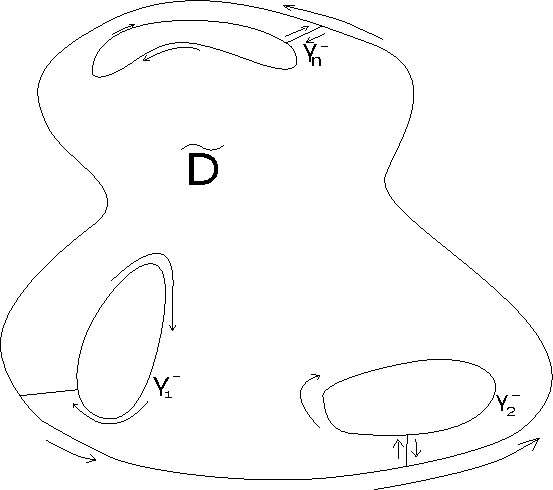
\includegraphics{fig1}
  \caption{Рисунок до доведення ~\ref{dov.8.4.1}}\label{fig.8.4.1}
\end{figure}

Отже рівність (8.2) доведена.
\end{dov}

\newpage

\subsection{Інтеграл і первісна.}\label{8.5}\allowdisplaybreaks

Нехай $D$ --- однозв'язна область, $f(z)$ --- аналітична в $D$, $z_0 \in D$ --- фіксована точка, $L_1$ і $L_2$ --- спрямлювані криві, які лежать в $D$ і з'єднують $z_0$ з довільною точкою $z \in D$. Якщо --- $L_2$ крива, яка проходиться від точки $z$ до точки $z$, то криві $L_1$ і --- $L_2$ складають замкнуту спрямлювану криву, і за інтегральною теоремою Коші:
\[ \int_{L_1}f(z)\,\mathrm{d}z + \int_{-L_2}f(z)\,\mathrm{d}z=0, \quad \text{або} \quad \int_{L_1}f(z)\,\mathrm{d}z=\int_{L_2}f(z)\,z \]

\begin{center}
  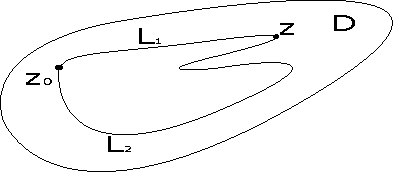
\includegraphics{fig2}
\end{center}

Тобто, значення інтеграла від аналітичної функції $f(z)$ не залежить від кривої, по якій проводиться інтегрування, а залежить тільки від початкової і кінцевої точок цієї кривої. Нехай точка $z_0$ фіксована, тоді інтеграл $\int_{z_0}^{z} f(\xi) \,\mathrm{d}\xi$ є функцією тільки від $z$, тобто
\begin{equation}\label{8.5.1}
\int_{z_0}^{z} f(\xi) \,\mathrm{d}\xi = F(z)
\end{equation}

Функція $F(z)$ диференційовна в області $D$ і $F'(z)=f(z)$. Доведемо дещо більш загальне твердження.

\begin{thm}\label{theor_8.5.1}
Нехай функція $f(z)$ неперервна в скінченній одноз'язній області $D$, і нехай інтеграл від $f(z)$ по довільній замкнутій кривій, яка лежить в області $D$, рівний нулю. Тоді функція $F(z)= \int_{z_0}^{z} f(\xi) \,\mathrm{d}\xi$ , де $z_0 \in D$, $z \in D$, диференційовна в області $D$ , тобто
\[ \left(\int_{z_0}^{z} f(\xi) \,\mathrm{d}\xi\right)' = f(z) \]

\end{thm}

\begin{proof}
При умовах теореми інтеграл  \(\int_{\gamma} f(\xi) \,\mathrm{d}\xi \) не залежить від кривої $\gamma$, яка лежить в області $D$ і з'єднує точки $z_0$ і $z$, а, значить, функція
\[ F(z) = \int_{z_0}^{z} f(\xi) \,\mathrm{d}\xi \]

однозначна в області $D$. Для точки $z+ \Delta z\in D$, яка лежить в околі точки $z \in D$, різниця
\[ \gamma = \frac{F(z+\Delta z)-F(z)}{\Delta z} - f(z) \longrightarrow 0 \quad \text{при} \quad \Delta z \rightarrow 0. \]

Покажемо це. Очевидно
\begin{equation}\label{8.5.2}
\frac{F(z+\Delta z) - F(z)}{\Delta z} = \frac{1}{\Delta z} \left\{ \int_{z_0}^{z+\Delta z} f(\xi) \,\mathrm{d}\xi - \int_{z_0}^{z} f(\xi) \,\mathrm{d}\xi \right\} = \frac{1}{\Delta z} \int_{z}^{z+\Delta z} f(\xi) \,\mathrm{d}\xi.
\end{equation}

Так як $\int_{z}^{z+\Delta z} f(\xi) \,\mathrm{d}\xi = \Delta z $ , то

\begin{equation}\label{8.5.3}
f(z) = \frac{f(z)}{\Delta z} \int_{z}^{z+\Delta z} \,\mathrm{d}\xi = \frac{1}{\Delta z} \int_{z}^{z+\Delta z} f(z) \,\mathrm{d}\xi
\end{equation}

Оскільки інтеграл в (\ref{8.5.2}) і (\ref{8.5.3}) незалежать від шляху по якому проводяться інтегрування, то візьмемо за шлях інтегрування відрізок, який з'єднує точки $z$ і $z+\Delta z$. Будемо мати

\[ \gamma = \frac{1}{\Delta z} \int_{z}^{z+\Delta z}\bigg[ f(\xi) - f(z) \bigg] \,\mathrm{d}\xi \text{,} \]

або
\begin{equation}\label{8.5.4}
|\gamma| \leq \frac{1}{|\Delta z|} \int_{z}^{z+\Delta z}\bigg| f(\xi) - f(z) \bigg|\cdot|d\xi|
\end{equation}

З неперервності функції $f(z)$ в області $D$, а значить і в точці $z\in D$ для $\\ \forall\epsilon > 0 \exists \delta = \delta(\epsilon) > 0$ таке, що при $|z-\xi|<\delta$ справджується нерівність
\begin{equation}\label{8.5.5}
|f(z)-f(\xi)|<\epsilon
\end{equation}

Ясно, що $|z-\xi|\leq |\Delta z|$, бо $\xi$ в (\ref{8.5.4}) належить відрізку $[z, z+\Delta z]$, тому (\ref{8.5.5}) буде виконуватися при $|\Delta z| < \delta$, а значить
\[ |\gamma| = \frac{1}{\Delta z} \cdot \epsilon \cdot |\Delta z|  \]

Таким чином існує
\[ \lim_{\Delta z\to 0}\frac{F(z+\Delta z)-F(z)}{\Delta z}=f(z) \text{,} \]

тобто $F'(z)=f(z)$
\end{proof}

Нехай функція $f(z)$ означена в області $D$, а функція $F(z)$ визначена рівністю (\ref{8.5.1}),  визначена в цій області.

\begin{ozn}
Якщо $F'(z)=f(z)$ для $\forall z\in D$, то функція $F(z)$ називається первісною функції $f(z)$ в області $D$.
\end{ozn}

Як бачимо, поняття первісної для функцій комплексного змінного вводиться таким де чином, як для функцій дійсного змінного.

З означення первісно і теореми \ref{theor_8.5.1} маємо, що $F(z)= \int_{z_0}^{z} f(\xi) \,\mathrm{d}\xi$ є первісною функції $f(z)$

\begin{thm}\label{theor_8.5.2}
Якщо функція $f(z)$ диференційовна в скінченній однозв'язній областв $D$, то вона має в $D$ первісну $F(z)$.
\end{thm}

\begin{proof}
Функція $f(z)$ задовольняє умови теореми \ref{theor_8.5.1}. Тому за цією теоремою функція $F(z)= \int_{z_0}^{z} f(\xi) \,\mathrm{d}\xi$ є первісною $f(z)$. Теорема доведена.
\end{proof}

\begin{thm}\label{theor_8.5.3}
Сукупність всіх первісних функції $f(z)$ в області $D$ визначається формулою $F_1(z)+C$, де $F_1(z)$ деяка первісна функції $f(z)$, а $C$ --- довільна стала
\end{thm}

\begin{dov}
Якщо $F_1(z)$ і $F_2(z)$ --- первісні функції $f(z)$ в області $D$, то функція $F(z)=F_2(z)-F_1(z)=u+iv$ є сталою в області $D$, бо за умовою $F'(z)=F_2'(z)- -F_1'(z)=f(z)-f(z)=0$ для $\forall z \in D$. А звідси слідує, згідно умови \emph{КРЕДа} (див. 5.4, формули (\ref{8.5.7}), (\ref{8.5.8})), що $\frac{\,\mathrm{d}u}{\,\mathrm{d}x}=\frac{\,\mathrm{d}v}{\,\mathrm{d}y}=\frac{\,\mathrm{d}u}{\,\mathrm{d}y}=\frac{\,\mathrm{d}v}{\,\mathrm{d}x}=0$ в області $D$, тобто $F(z)\equiv const$, або $F_2(z)=F_1(z)+C$, де $C$ --- комплексна стала.
\end{dov}

\begin{corollary}\label{corollary_8.5.1}
При умовах теореми \ref{theor_8.5.1}, або \ref{theor_8.5.2} довільна первісна $F(z)$ функції $f(z)$ виражається формулою
\begin{equation}\label{8.5.6}
F(z)= \int_{z_0}^{z}f(\xi)\,\mathrm{d}\xi + C, \quad \text{де $C$ --- комплексна стала.}
\end{equation}
\end{corollary}

\begin{corollary}\label{corollary_8.5.2}
При умовах теореми \ref{theor_8.5.1}, або \ref{theor_8.5.2} має місце формула Ньютона-Лейбніца
\begin{equation}\label{8.5.7}
\int_{z_0}^{z_1}f(\xi)\,\mathrm{d}\xi = F(z_1) - F(z_0)
\end{equation}
\end{corollary}
\begin{proof}
Якщо покласти в формулі (\ref{8.5.6}) $z=z_0$, то одержимо, що $F(z_0)=C$, а якщо --- $z=z_1$, то
\[F(z_1)=\int_{z_0}^{z_1}f(\xi)\,\mathrm{d}\xi + C = \int_{z_0}^{z_1}f(\xi)\,\mathrm{d}\xi + F(z_0). \]

Звідси слідує рівність (\ref{8.5.7}).
\end{proof}

\begin{corollary}\label{corollary_8.5.3}
Якщо функції $f(z)$ і $g(z)$ задовольняють умови теореми \ref{theor_8.5.2}, то справедлива формула інтегрування частинами:
\begin{equation}\label{8.5.8}
\int_{z_0}^{z_1} f(\xi)g'(\xi)\,\mathrm{d}\xi = \bigg[f(\xi)g(\xi)\bigg] \bigg|_{z_0}^{z_1}-\int_{z_0}^{z_1}f'(\xi)g(\xi)\,\mathrm{d}\xi.
\end{equation}
\end{corollary}
\begin{dov}
Оскільки $(f\cdot g)'=f'\cdot g + f \cdot g'$, то користуючись формулою (\ref{8.5.7}), будемо мати
\[ \int_{z_0}^{z_1}(fg)'\,\mathrm{d}\xi=f(\xi_1)\cdot g(\xi_1)-f(z_0)\cdot g(z_0) = [f(\xi)g(\xi)]\bigg|_{z_0}^{z_1}, \]
що доводить рівність (\ref{8.5.8}).
\end{dov}

В однозв'язній області інтеграли від диференційовних елементарних функцій комплексного змінного обчислюються з допомогою тих же і формул, що й у випадку дійсних функцій.

\begin{exm}\label{exm_8.5.1}
Функція $f(z)=\frac{1}{z}$ диференційовна в неоднозв'язній області $\\ D:0<|z|<\infty$. Якщо $ \widetilde{D}\subset D$ і $\widetilde{D}$ --- однозв'язна область. Функція
\[ F(z) = \int_{1}^{z} \frac{\,\mathrm{d}\xi}{\xi}, \quad z \in \widetilde{D}, \]

де інтеграл береться по довільній кривій, що лежить в $\widetilde{D_1}$ є первісною, згідно теореми \ref{theor_8.5.2}, для функції $\frac{1}{z}$ і $F'(z)=\frac{1}{z}$. Але функція
\[ \Phi (z)= \int_{1}^{z} \frac{\,\mathrm{d}\xi}{\xi}, \quad z \in D \]

є неоднозначною в області $D$, бо
\[ \int_{|z|=1} \frac{\,\mathrm{d}\xi}{\xi}=2\pi i \neq 0. \]
\end{exm}

\newpage

\section{Інтегральна формула Коші}\label{9}\allowdisplaybreaks

\subsection{Інтеграл Коші.}\label{9.1}
З інтегральної теореми Коші слідує одна з важливіших (і красивіших) формул теорії функцій комплексного змінного --- інтегральна формула Коші.
\begin{thm}[інтегральна формула Коші]
Нехай $f(z)$ --- функція однозначна і аналітична в області $D$ і $L$ --- замкнута жорданова спрямлювана крива, яка належить $D$ разом із своєю внутрішністю $G$. Тоді для будь-якої точки $z\in G$ справедлива інтегральна формула Коші.
\begin{equation}\label{9.1.1}
f(z)=\frac{1}{2\pi i}\int_{L}\frac{f(\xi)}{\xi - z}\,\mathrm{d}\xi, \quad z\in G.
\end{equation}

Тут крива $L$ проходиться в додатньому напрямі, тобто проти годинникової стрілки. Інтеграл в правій часті формули (\ref{9.1.1}) називають інтегралом Коші.
\begin{center}
  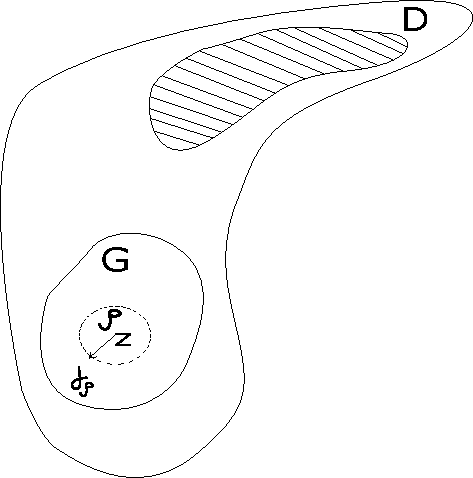
\includegraphics{fig3}
\end{center}
\end{thm}
\begin{dov}\label{dov.9.1.1}
Опишемо з точки $z$, як з центра, коло $\gamma_\rho$ настільки малого радіуса $\rho$, щоб воно містилось в $L$. Тоді для контура, утвореного кривими $L$ і $\gamma_\rho$, будемо мати:
\begin{equation}\label{9.1.2}
\frac{1}{2\pi i}\int_{L}\frac{f(\xi)\,\mathrm{d}\xi}{\xi-z} = \frac{1}{2\pi i}\int_{\gamma_\rho} \frac{f(\xi)\,\mathrm{d}\xi}{\xi-z}
\end{equation}
Для доведення формули (\ref{9.1.1}) достатньо встановити рівність
\[ f(z)= \frac{1}{2\pi i} \int_{L}\frac{f(\xi)\,\mathrm{d}\xi}{\xi-z} \]
або рівність
\begin{equation}\label{9.1.3}
\int_{\gamma_\rho}\frac{f(\xi)}{\xi-z}\,\mathrm{d}\xi=2\pi if(z) = \int_{\gamma_\rho}\frac{f(\xi)}{\xi-z}\,\mathrm{d}\xi-f(z)\int_{\gamma_\rho}\frac{d\xi}{\xi-z}=\int_{\gamma_\rho}\frac{f(\xi)-f(z)}{\xi-z}\,\mathrm{d}\xi=0.
\end{equation}
Внаслідок неперервності функції $f(\xi)$ в точці $z$ нерівність
\[ |f(\xi)-f(z)|<\epsilon, \quad \xi\in\gamma_\rho \]

буде виконуватись для $\forall\epsilon>0$, якщо $\rho<\delta=\delta(\epsilon)$. Тому
\[ \bigg| \int_{\gamma_\rho} \frac{f(\xi)-f(z)}{\xi-z}\,\mathrm{d}\xi \bigg|< \frac{\epsilon}{\rho} 2\pi\rho=2\pi\epsilon. \]
А значить
\[ \lim_{\rho \to 0} \int_{\gamma_\rho} \frac{f(\xi)-f(z)}{\xi-z}\,\mathrm{d}\xi=0. \]

Інтеграл $\int_{\gamma_\rho} \frac{f(\xi)}{\xi - z}\,\mathrm{d}\xi$ не залежить від $\rho$, що видно з рівності (\ref{9.1.2}), а інтеграл $\int_{\gamma_\rho} \frac{f(\xi)-f(z)}{\xi - z}\,\mathrm{d}\xi$ також не залежить від $\rho$. Значить він рівний нулю при всіх $\rho < \delta(\epsilon)$. Таким чином рівність (\ref{9.1.3}) справедлива і інтегральна формула Коші (\ref{9.1.1}).
Значення функції $f(z)$ всередині області виражається з допомогою формули (\ref{9.1.3}) через її значення цієї області.

Нехай функція $f(z)$ диференційовна в області $D$, а $\gamma_1$ і $\gamma_2$ --- жорданові спрямлювальні криві ($\gamma_1$ лежить всередині $\gamma_2$), які утворюютть границю області $D_1 \subset D$ (див. рис. \ref{fig.9.1.1}). Тоді для $\forall z \in D_1$ справедлива формула
\begin{equation}\label{9.1.4}
f(z)=\frac{1}{2\pi i}\int_{\gamma_2}\frac{f(\xi)}{\xi-z}\,\mathrm{d}\xi-\frac{1}{2\pi i}\int_{\gamma_1}\frac{f(\xi)}{\xi-z}\,\mathrm{d}\xi
\end{equation}
При обході кривих $\gamma_2$ і $\gamma_1$ внутрішністю кожної з них залишається зліва.
\begin{figure}
  \centering
  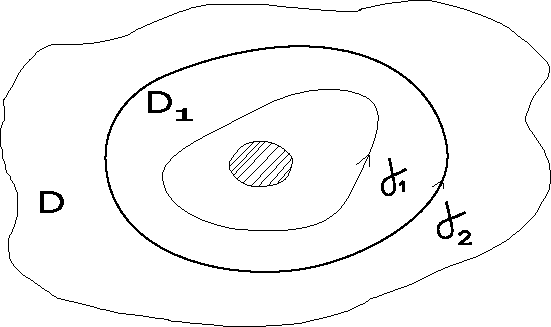
\includegraphics{fig4}
  \caption{Рисунок до доведення \ref{dov.9.1.1}}\label{fig.9.1.1}
\end{figure}
\end{dov}


\begin{remark}\label{remark_9.1.1}
Якщо в правій частині формули (\ref{9.1.3}) $z$ належить зовнішності кривої $\Gamma$, тобто $z \in \bar{D}$, то підінтегральна функція диференційовна по $\xi$ скрізь в $D$ і за теоремою Коші інтеграл рівний нулю, тобто

\[ \frac{1}{2\pi i} \int_{\Gamma} \frac{f(\xi)}{\xi-z}\,\mathrm{d}\xi= \bigg\{ \begin{matrix} f(z), \quad z\in D \\ 0, \quad z \in D \end{matrix} \]

\end{remark}

\subsection{Теорема про середнє.}\label{9.2}
Теорема про середнє. Якщо функція $f(z)$ диференційовна в крузі $K:|z-z_0|<R$ і неперервна в замкнутому крузі $\bar{K}$, то значення цієї функції в центрі круга рівне середньому арифметичному її значень на колі, тобто
\begin{equation}\label{9.2.1}
f(z_0)=\frac{1}{2\pi}\int_{0}^{2\pi}f(z_0+Re^{i\varphi})\,\mathrm{d}\varphi.
\end{equation}

\begin{dov}
Якщо в формулі (\ref{9.1.1}) взяти $L$ як коло радіуса $R$ з центром в точці $z_0$, тобто
\[ L: \xi=z_0+Re^{i\varphi},\quad 0\leq\varphi\leq2\pi,\quad \text{то} \]
\[ f(x)=\frac{1}{2\pi}\int_{L}\frac{f(\varphi)}{\xi-z_0}\,\mathrm{d}\xi = \frac{1}{2\pi i} \int_{0}^{2\pi}\frac{f(z_0+Re^{i\varphi})iRe^{i\varphi}}{Re^{i\varphi}}\,\mathrm{d}\varphi. \]

Що й доводить формула (\ref{9.2.1}).
\end{dov}

\end{document} 